%!TEX root = ../dokumentation.tex
\chapter{Results}\label{results}

The test runs that were done for a total of 708 different configurations with 236 different configurations for each solver. They were run twice for each configuration and the results where aggregated by calculating the mean. Nonetheless, only 649 configurations were recorded for which at least one of the runs was successful. And every single one of the 59 unsuccessful runs was a run using the "inverse" solver. In particular the $\acs{ARIMA}(2,1,2)$ and  $\acs{ARIMA}(4,1,4)$ models were crashing for all time series with sizes starting from $50,000$ and the $\acs{MA}(3)$ and $\acs{MA}(6)$ models were \textit{mostly} not working for time series with sizes starting from $150,000$. However, for the 649 configurations that were producing results, the maximal difference between the \acl{CSS} that the R script calculated and that of the \acs{DML} script was only $5e^{-13}$ and the mean difference was $4e^{-14}$. As the results of both the R and the \acs{DML} script are only returning results with up to 16 decimal places, the minimal non-zero difference that could have been measured is $1e^{-16}$. Therefore there is no further need to examine the distribution of these computational errors.

However, the data collected on the performance of the algorithms is more complex by far. Hence, the following presentation of the performance measurements is structure in a way that first introduces the results in a reasonably general way and then drills further down into the details by showing the data with respect to the following six dimensions:
\begin{enumerate}
    \item \textbf{Script type and solvers}: Whether the results are from the \acs{DML} or R script and which type of solver was used in the \acs{DML} script.
    \item \textbf{Time measurement}: Whether the measurement was recording the execution time or the run time as described in chapter \ref{performance_precision_testing}
    \item \textbf{Time series category}: Whether the time series is part of the group of "small" or "large" time series. Small scale time series are defined as time series with sizes smaller or equal to $1,000$ and large scale time series are defined as time series with sizes greater than $1,000$
    \item \textbf{Model class}: Whether the data describes an \acs{AR}, \acs{MA} or \acs{ARIMA} model
    \item \textbf{Model}: The exact model specified by its class and the order of the model. Data includes $\acs{AR}(3)$, $\acs{AR}(6)$, $\acs{MA}(3)$, $\acs{MA}(6)$, $\acs{ARIMA}(2,1,2)$ and $\acs{ARIMA}(4,1,4)$ models.
    \item \textbf{Time series size}: The actual size in terms of number of observations
\end{enumerate}

In its most comprehensive form the results of the performance tests are presented in figure \ref{fig:stats-mean-execandrun-allscripts} which shows the mean values of the execution and run time for all four script types while also differentiating the two time series size categories. From this representation alone, there are already 3 important properties of the test results that can be observed:

\begin{enumerate}
    \item On average R is faster than any one of the three DML scripts. The only exception is the run time for small scale time series which is roughly three times slower than the fastest DML script. However, the difference of the other three values is much greater. On small scale with a factor of at least 15 and on large scale with a factor of at least 40 for run time and a factor of 140 for the execution time.
    \item Generally the difference between execution and run time is greater for small scale time series than for large scale time series. For the DML scripts the difference is smaller than 1\% for large scale time series and therefore insignificant. For R, on the other hand, the difference is significant independent of the time series’ size.
    \item Of the three DML scripts, the inverse one is the slowest by a huge margin. Both the Jacobi and Forward Substitution solver are more than twice as fast on average. Of these two, the Jacobi solver is 4.5\% faster on average.
\end{enumerate}

For the further presentation of the results this means that, first of all, the dimension of \textit{time measurement} will be reduced to one element only - the execution time - for all comparisons that are focused on the model or solver dimension and secondly that the DML script with the inverse solver won't be the subject of any more detailed presentation as it is already obvious that it is considerably worse for large scale time series compared to all the other scripts and not significantly better on small scale. Note that, even though these parts of the results are not discussed in this chapter, there are additional tables and plots of a wider variety of views in appendix \ref{AppendixA}.

\begin{table}[!htbp]
    \centering
    \begin{tabular}{|C{2.4cm}||r|r||r|r|r|}
        \hline
        \multirow{ 2}{*}{Script} & \multicolumn{1}{c|}{execution time} & \multicolumn{1}{c||}{run time} & \multicolumn{1}{c|}{execution time} & \multicolumn{1}{c|}{run time} \\ 
        \cline{2-5}
        & \multicolumn{2}{c||}{small scale} & \multicolumn{2}{c|}{large scale}\\
        \hline\hline
        Inverse DML  & 1.24 & 3.15  & 1,767.3 & 1,769.44 \\
        \hline
        Forwardsub DML & 1.21 & 4.74  & 528.43 & 530.82 \\
        \hline
        Jacobi DML& 1.35 & 4.59  & 505.81 & 508.47 \\
        \hline
        R  & 0.08 & 9.67  & 3.65 & 11.95 \\
        \hline
    \end{tabular}
     \caption{Comparison of \textbf{execution and run time} mean values of \textbf{DML and R} implementations for \textbf{small scale} (from $50$ to $1,000$) and \textbf{large scale} (from $50,000$ to $950,000$) time series}
    \label{fig:stats-mean-execandrun-allscripts}
\end{table}

The next three figures \ref{fig:stats-jacobi-dml-exectime}, \ref{fig:stats-forwardsub-dml-exectime}, and \ref{fig:stats-r-exectime} show the statistical characteristics of the execution time in more detail by expanding the view on the data with the dimension of the model classes.  

When comparing these tables with respect to the \acl{AR} models one can see that there is an average increase in execution time from small scale to large scale by factor of 5 for Jacobi, a factor of 15 for Forward Substitution and a factor of 75 for R. With the average large scale time series having 1000 times more observations than an average small scale time series. For small scale time series, Jacobi and Forward Substitution are pretty close in terms of their mean execution time, with Jacobi taking 10.8\% less time. The absolute difference, however, is only 1/10 of a second. When comparing the execution time R is 13 times faster than Jacobi. However, this is not the case for the run time, because using the \acs{HDFS} has a much grater impact on the performance of R than on DML. Therefore the run time of DML for small scale \acs{AR} models is twice as good (see additional run time statistics \ref{apx-fig:stats-allmodels-dml-runtime-small} and \ref{apx-fig:stats-allmodels-r-runtime-small}). This is true for the averages of all model classes. For large scale time series Jacobi has the best average execution time. It even takes 15\% less time than R to produce the results. And it is more than 3 times faster than the script using Forward Substitution 


For the \acl{MA} models the difference between small scale and large scale is much greater than for the \acs{AR} models. For the Jacobi and Forward Substitution scripts there is more than a 150 fold increase while the increase of R is only 18 fold. And both on small and large scale the R script is absolutely outperforming any of the DML implementations. For small scale it is 16 times faster than Forward Substitution, which itself takes 16\% less time than Jacobi. For large scale R is even better than that with an average of 1.5 seconds to 226 seconds for Forward Substitution and 235 seconds for Jacobi, making it more than 150 times faster than any one of them. An interesting fact to note here is that the execution time of R for large scale time series with the \acl{AR} model is 4 times that of the \acl{MA} model. 

For the complete \acl{ARIMA} model there is an average increase in execution time from small to large scale by a factor of 955 for Jacobi and by 1227 for Forward Substitution. This is a huge difference. But note that for large scale time series the maximal value measured for both solvers is roughly 3 times the mean value. On the other hand, for the class of \acs{MA} models the maximal execution time was only about 1.4 times the mean. The increase for R from small to large scale is only 45 fold and with an average execution time of only 3.6 seconds for large scale time series the R script is 370 times faster than any one of the DML scripts. Of the two DML scripts the script using the Jacobi solver is the faster one. But again the difference is only about 4\%, making it statistically insignificant.


\begin{table}[!htbp]
    \centering
    \begin{tabular}{|C{2cm}||r|r|r||r|r|r|}
        \hline
        \multirow{ 2}{*}{Stat.} & \multicolumn{1}{c|}{AR} & \multicolumn{1}{c|}{MA} & \multicolumn{1}{c||}{ARIMA} & \multicolumn{1}{c|}{AR} & \multicolumn{1}{c|}{MA} & \multicolumn{1}{c|}{ARIMA} \\ 
        \cline{2-7}
        & \multicolumn{3}{c||}{small scale} & \multicolumn{3}{c|}{large scale}\\
        \hline\hline
        \rowcolor{lightGray}
        min & 0.47 & 0.5 & 0.46 & 1.27 & 20.4 & 10.09 \\
        \hline
        max & 2.32 & 3.25 & 3.16 & 10.64 & 340.35 & 4,091.19 \\
        \hline
        \rowcolor{lightGray}
        mean & 1.08 & 1.54 & 1.42 & 5.15 & 235.05 & 1,356.96 \\
        \hline
        median & 1.06 & 1.23 & 1.04 & 4.46 & 253.88 & 1,006.21 \\
        \hline
        \rowcolor{lightGray}
        standard deviation & 0.45 & 0.89 & 0.87 & 2.89 & 72.9 & 1,159.36 \\
        \hline
    \end{tabular}
     \caption{Statistical analysis of \textbf{DML execution time} for \textbf{small scale} (from $50$ to $1,000$) and \textbf{large scale} (from $50,000$ to $950,000$) time series for \textbf{Jacobi solver}}
    \label{fig:stats-jacobi-dml-exectime}
\end{table}

\begin{table}[!htbp]
    \centering
    \begin{tabular}{|C{2cm}||r|r|r||r|r|r|}
        \hline
        \multirow{ 2}{*}{Stat.} & \multicolumn{1}{c|}{AR} & \multicolumn{1}{c|}{MA} & \multicolumn{1}{c||}{ARIMA} & \multicolumn{1}{c|}{AR} & \multicolumn{1}{c|}{MA} & \multicolumn{1}{c|}{ARIMA} \\ 
        \cline{2-7}
        & \multicolumn{3}{c||}{small scale} & \multicolumn{3}{c|}{large scale}\\
        \hline\hline
        \rowcolor{lightGray}
        min & 0.58 & 0.5 & 0.52 & 1.98 & 20.42 & 9.04 \\
        \hline
        max & 2.2 & 4.5 & 2.3 & 42.6 & 315.31 & 4,049.64 \\
        \hline
        \rowcolor{lightGray}
        mean & 1.19 & 1.28 & 1.16 & 18.66 & 226.39 & 1,423.5 \\
        \hline
        median & 1.11 & 0.99 & 1.17 & 17.4 & 239.03 & 1,113.43 \\
        \hline
        \rowcolor{lightGray}
        standard deviation & 0.47 & 0.9 & 0.53 & 12.01 & 71.71 & 1,090.63 \\
        \hline
    \end{tabular}
     \caption{Statistical analysis of \textbf{DML execution time} for \textbf{small scale} (from $50$ to $1,000$) and \textbf{large scale} (from $50,000$ to $950,000$) time series for \textbf{Forward-substitution solver}}
    \label{fig:stats-forwardsub-dml-exectime}
\end{table}


\begin{table}[!htbp]
    \centering
    \begin{tabular}{|C{2cm}||r|r|r||r|r|r|}
        \hline
        \multirow{ 2}{*}{Stat.} & \multicolumn{1}{c|}{AR} & \multicolumn{1}{c|}{MA} & \multicolumn{1}{c||}{ARIMA} & \multicolumn{1}{c|}{AR} & \multicolumn{1}{c|}{MA} & \multicolumn{1}{c|}{ARIMA} \\ 
        \cline{2-7}
        & \multicolumn{3}{c||}{small scale} & \multicolumn{3}{c|}{large scale}\\
        \hline\hline
        \rowcolor{lightGray}
        min & 0.05 & 0.05 & 0.05 & 0.57 & 0.24 & 0.4 \\
        \hline
        max & 0.19 & 0.17 & 0.17 & 13.03 & 3.21 & 7.71 \\
        \hline
        \rowcolor{lightGray}
        mean & 0.08 & 0.08 & 0.08 & 6.07 & 1.49 & 3.65 \\
        \hline
        median & 0.07 & 0.07 & 0.06 & 6.32 & 1.3 & 3.51 \\
        \hline
        \rowcolor{lightGray}
        standard deviation & 0.03 & 0.03 & 0.03 & 3.31 & 0.87 & 2.22 \\
        \hline
    \end{tabular}
     \caption{Statistical analysis of \textbf{R execution time} for \textbf{small scale} (from $50$ to $1,000$) and \textbf{large scale} (from $50,000$ to $950,000$) time series}
    \label{fig:stats-r-exectime}
\end{table}

So far the data was analyzed only on the first four dimensions: Script type and solvers, time measurement, time series category and model classes. In the following section of this chapter, the results are more closely looked at with regards to the last two dimensions time series size and model. 

First, have a look at the scatter plots of figures \ref{fig:ar-comparison-jacobi}, \ref{fig:ma-comparison-jacobi} and \ref{fig:arima-comparison-jacobi}. They show how different models of the same model class are comparing to each other in terms of their execution time for large scale time series and the Jacobi solver. 

In case of the class of \acl{AR} processes the two models are actually extremely closely correlated with a correlation of $r=0.91$. What is most interesting about this is that even the measurements that look like they might be outliers, for example the observations for $450k$ and $550k$, still show this correlation. Of these 40 data points there is actually only two, the measurements for $800k$, that do not look like they are tightly correlated. Also note that the two trend lines that have been plotted show that, surprisingly, it is the $\acs{AR}(3)$ model that appears to be slightly better.

For the other two model classes \acs{MA} and \acs{ARIMA} there is no significant linear correlation. The correlation of the \acl{MA} models is only $r=0.55$ and the correlation of the \acs{ARIMA} models is even less with $r=0.47$. However, for the class of \acs{MA} processes one can clearly see, that the correlation could have been much better for most parts of the data. Especially for the measurements of time series with sizes greater than $400k$. There the correlation is $0.91$. And for the time series from $1k$ to $250k$ the correlation is even $0.94$. Just from looking at the graph \ref{fig:ma-comparison-jacobi} one can't tell that the the observations that are reducing the overall correlation so significantly are not part of the underlying pattern that seems to emerge from the rest of the data. Disregarding these abnormalities for a moment, the pattern mentioned is quite interesting as it is not simply linear. For the first few observations the measurements of each model look like they might be described with a quadratic function, but then the pattern abruptly changes to a linear model at the $150k$ mark. Note that from the linear trend lines that are shown in the plot one can clearly see that for the class of \acl{MA} models the higher order models take more time to compute.

In contrast to that, the correlation of the \acs{ARIMA} models execution time does not seem like it might have been corrupted by a few outliers. However, the standard deviation for the \acs{ARIMA}(4,1,4) model is significantly greater than the one for \acs{ARIMA}(2,1,2). To be more precise, the standard deviation of the higher order model is 16 times greater (see appendix \ref{apx-fig:stats-allmodels-jacobi-dml-exectime-big}).  But this is only one factor that explains the low linear correlation. By comparing the linear trends of the two \acs{ARIMA} models one can also see, that they are diverging greatly with increasing time series size, with the higher order model \acs{ARIMA}(4,1,4) being the one taking longer and longer for each increase in time series size.

\begin{figure}[!ht]
	\centering
	\scalebox{1}{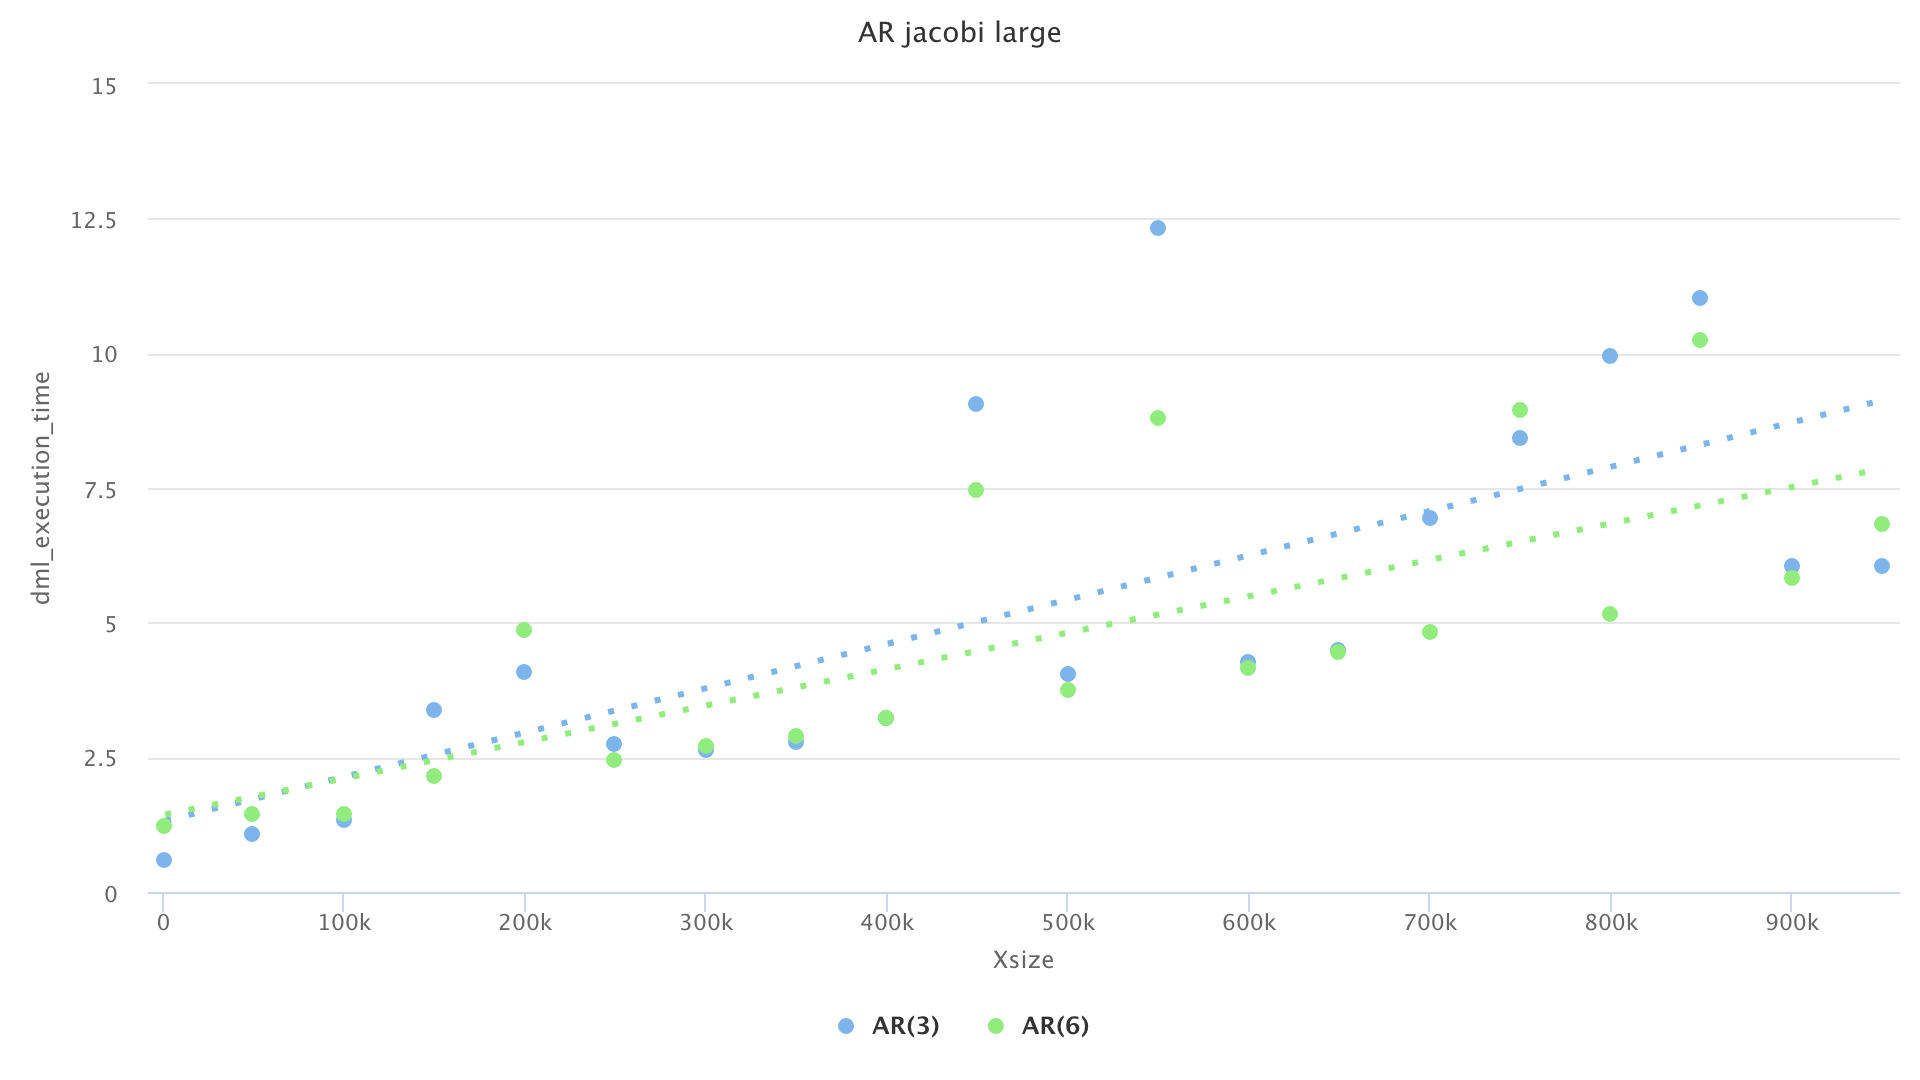
\includegraphics[width=\thirdsizeGraph]{images/ar-comparison-jacobi_large.png}}
	\caption{Comparison of \textbf{Execution time} of \textbf{AR(3) and AR(6) for Jacobi-DML} for time series with sizes \textbf{from $1,000$ up to $950,000$} }
    \label{fig:ar-comparison-jacobi}
\end{figure}

\begin{figure}[!ht]
	\centering
	\scalebox{1}{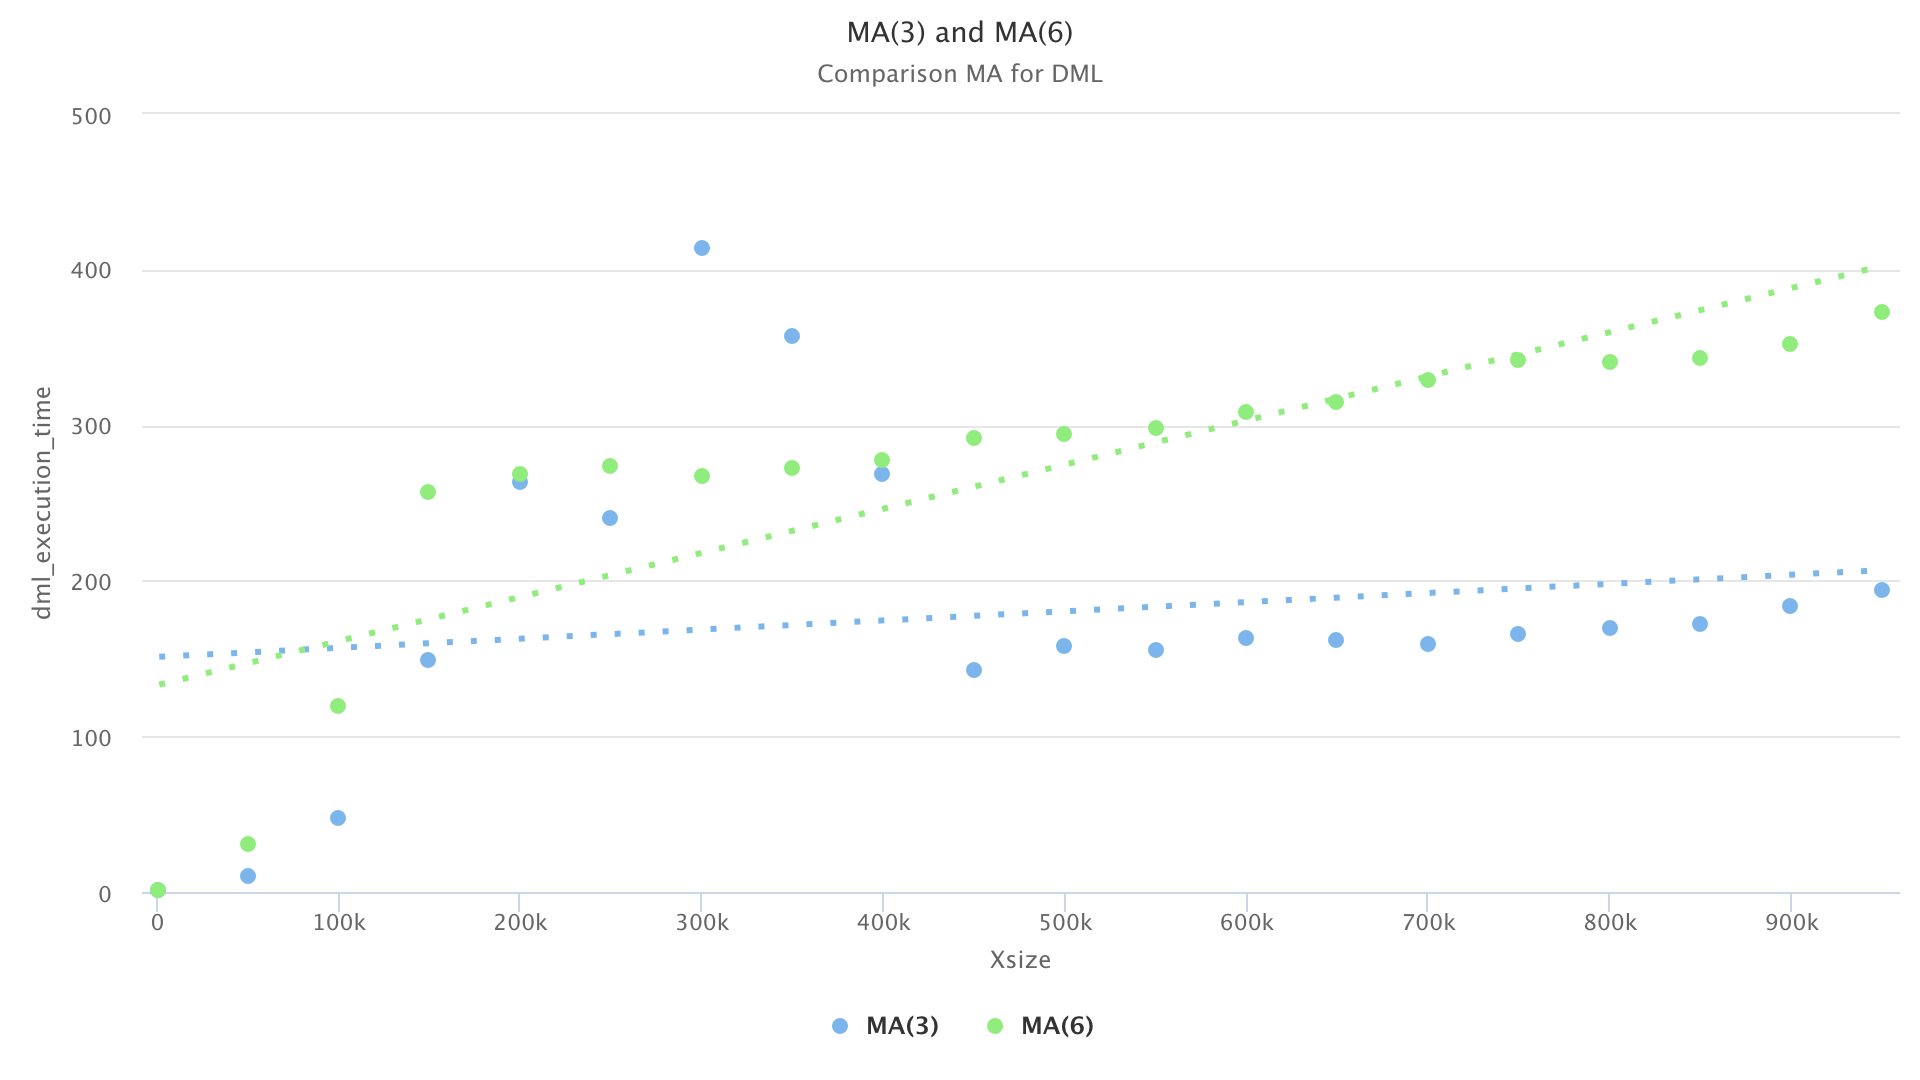
\includegraphics[width=\thirdsizeGraph]{images/ma-comparison_jacobi.png}}
	\caption{Comparison of \textbf{Execution time} of \textbf{MA(3) and MA(6) for Jacobi-DML} for time series with sizes \textbf{from $1,000$ up to $950,000$} }
    \label{fig:ma-comparison-jacobi}
\end{figure}

\begin{figure}[!ht]
	\centering
	\scalebox{1}{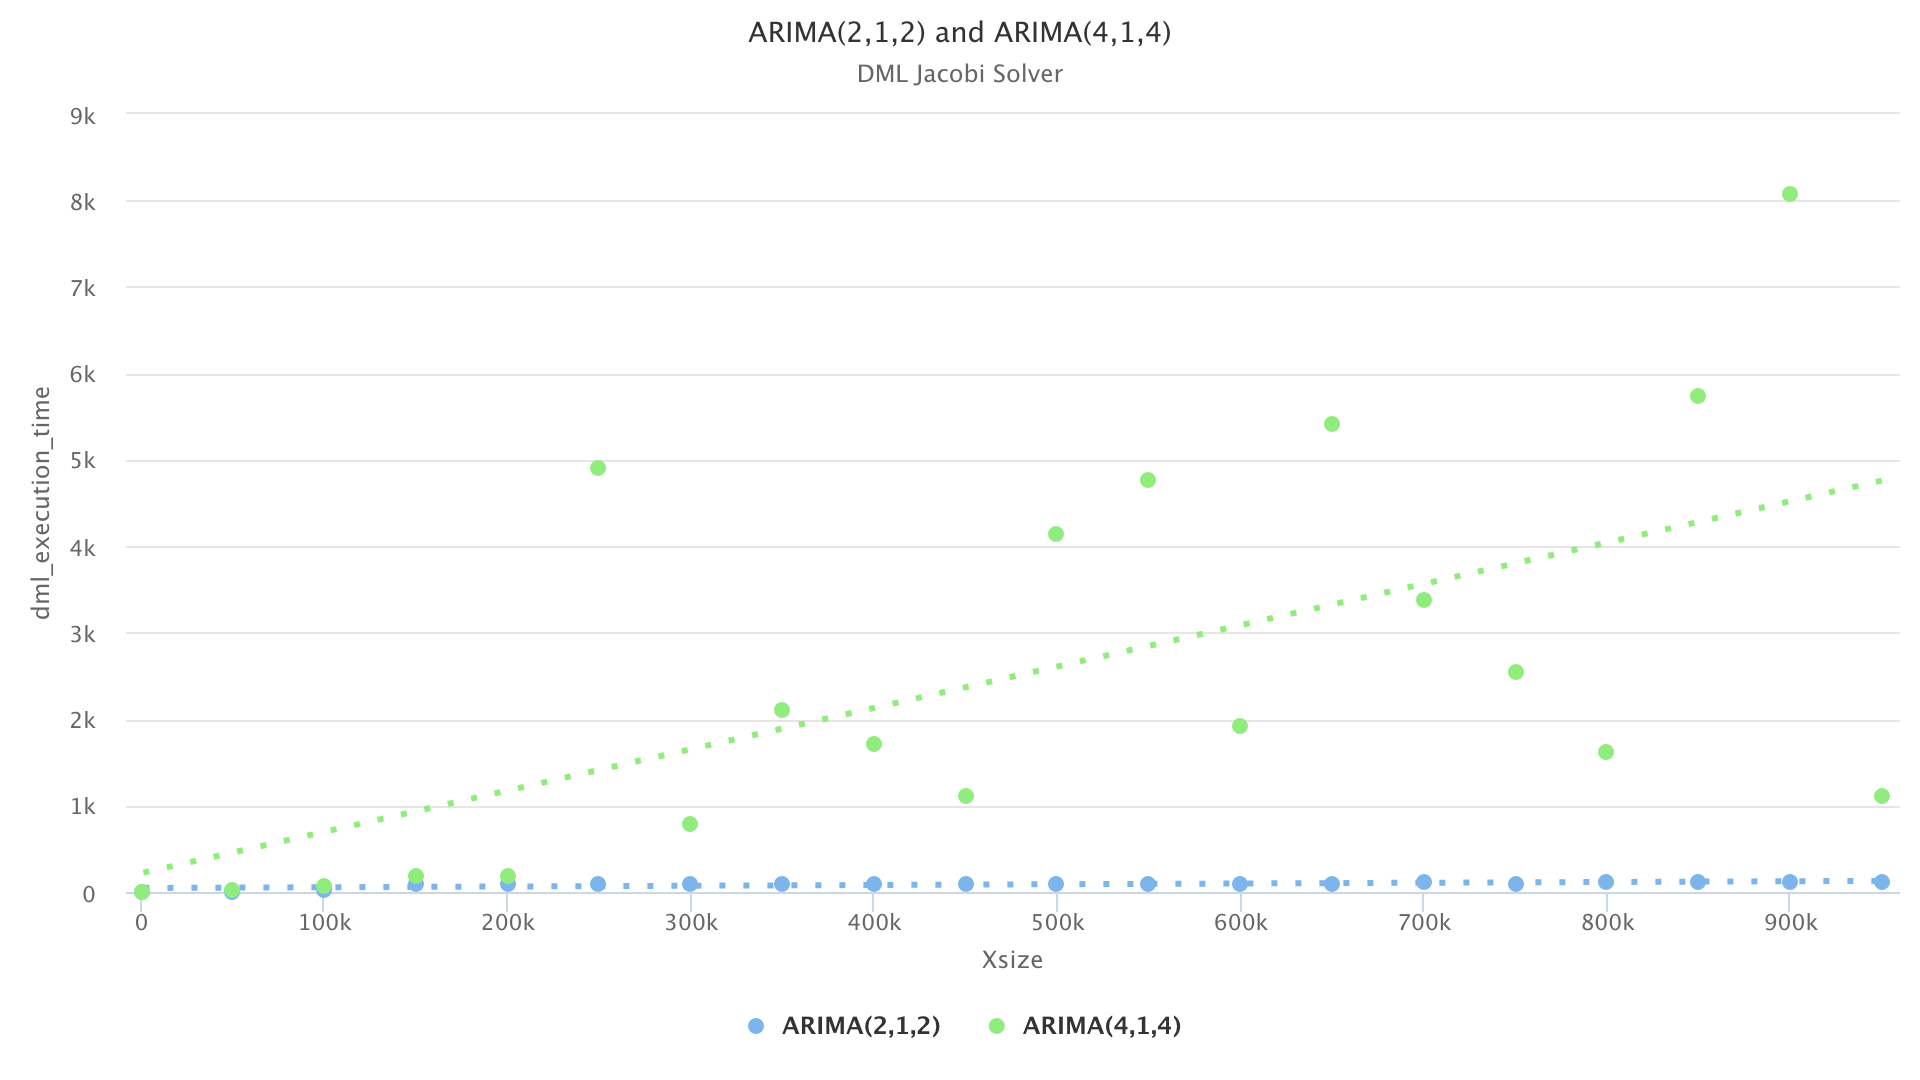
\includegraphics[width=\thirdsizeGraph]{images/arima-comparison_jacobi.png}}
	\caption{Comparison of \textbf{Execution time} of \textbf{ARIMA(2,1,2) and ARIMA(4,1,4) for Jacobi-DML} for time series with sizes \textbf{from $1,000$ up to $950,000$} }
    \label{fig:arima-comparison-jacobi}
\end{figure}



The next two plots show the execution time dependent on the time series size for all four solvers and scripts. The first figure \ref{fig:ar3-exectime-scatter-all-regression} for \acs{AR}(3) and the second one, figure \ref{fig:ma3-exectime-scatter-all_reduced-regression}, for \acs{MA}(3). 

For the \acl{AR} model the data that can be seen in figure \ref{fig:ar3-exectime-scatter-all-regression} is pretty straight forward. As was discussed in the beginning of this chapter: The inverse solver is completely off the charts, the Forward Substitution solver is slower than Jacobi and R, and the Jacobi solver is insignificantly better than R. Almost surprisingly there are no outliers or any other kind of unexpected patterns in the data. 

This is definitely not the case for figure \ref{fig:ma3-exectime-scatter-all_reduced-regression} showing the \acs{MA}(3) model. As it could already be seen in one of the previous figures showing the class of \acl{MA} models, there is a significant set of observations that absolutely don't fit any obvious patterns. And what is most interesting about these observations ranging from $150k$ to $400k$ is that they first of all, are so much bigger than the following measurements and more importantly are occurring both for the Jacobi solver and the Forward Substitution solver, but not for the Inverse solver or for R. Setting these outliers a side again, one can see that the two approaches Jacobi and Forward Solver are equally good, but not comparable to the performance of R's implementation. 

The plots describing the execution time of \acs{ARIMA}(2,1,2) show similar characteristics as the one for \acl{MA}(3). The first figure \ref{fig:arima212-exectime-scatter-all-regression} demonstrates the scale of the measurements and mainly shows why the mean value for the \acs{ARIMA} models is so high. There are three outliers that impacted the mean disproportional. As mentioned before the maximal value for \acs{ARIMA} was roughly 3 times the mean value. Removing only the three largest outliers results in a representation of the data as it can be seen in figure \ref{fig:arima212-exectime-scatter-all} and would mean an average execution time of only 90.45 seconds. As one would expect, the same pattern that could be observed for the \acl{MA} models is also being exhibited by the \acs{ARIMA}(2,1,2) process. For the values from $1k$ up to $150k$ the patterns seems to be of a quadratic function, but then breaks and continues in the form of a linear model which also looks to be quite stable, if one is willing to disregard the outliers. These linear models are shown in figure \ref{fig:arima212-exectime-scatter-all-excludeOutlier-regression}. From looking at this last figure one can see that the Forward Substitution solver seems to be the slower one for increasing sizes in the time series. However, this difference is quite small and the trend lines based only on small set of observations. And finally, each one of these figures also shows that the implementation of R is much faster than any DML implementations.

\begin{figure}[ht]
	\centering
	\scalebox{1}{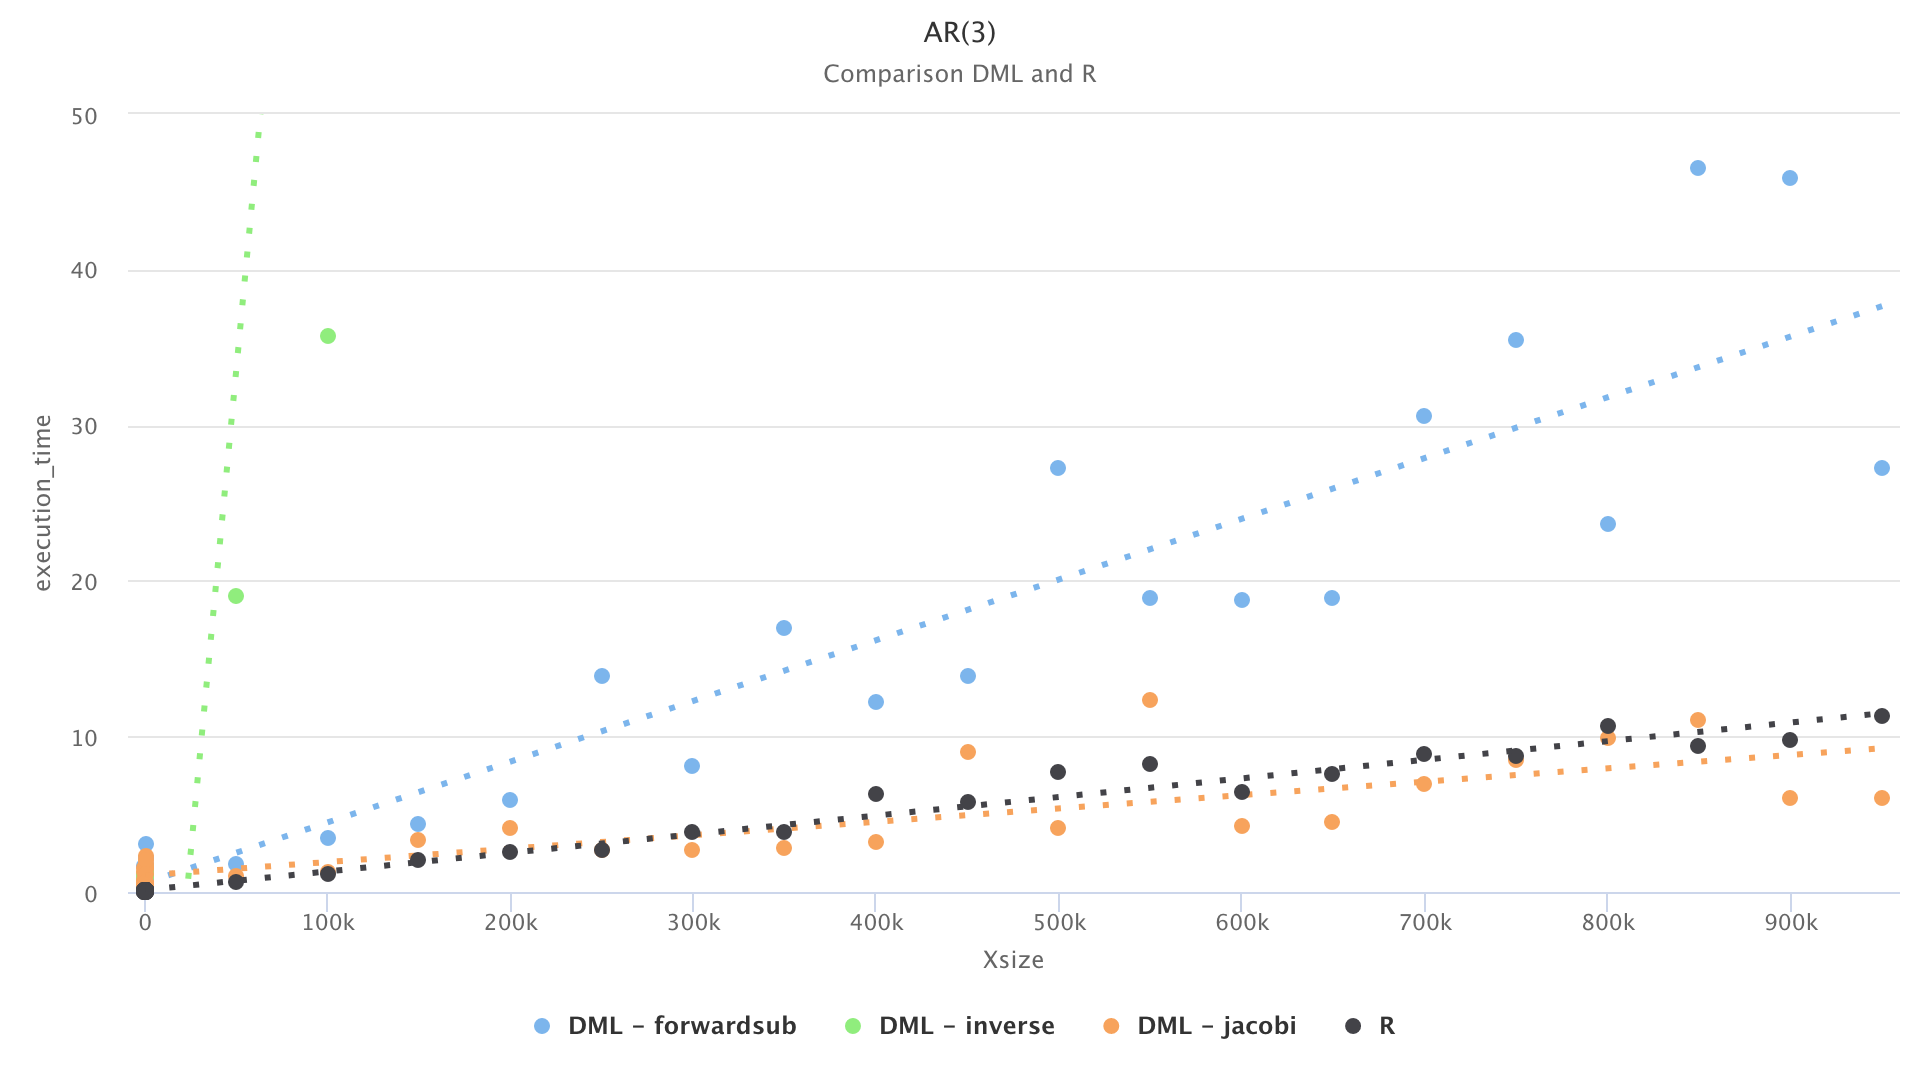
\includegraphics[width=\defaultsizeGraph]{images/ar3-exectime-scatter-all-regression.png}}
	\caption{\textbf{Execution time} of AR(3) for DML and R for time series with sizes \textbf{up to $950,000$} }
    \label{fig:ar3-exectime-scatter-all-regression}
\end{figure}

\begin{figure}[ht]
	\centering
	\scalebox{1}{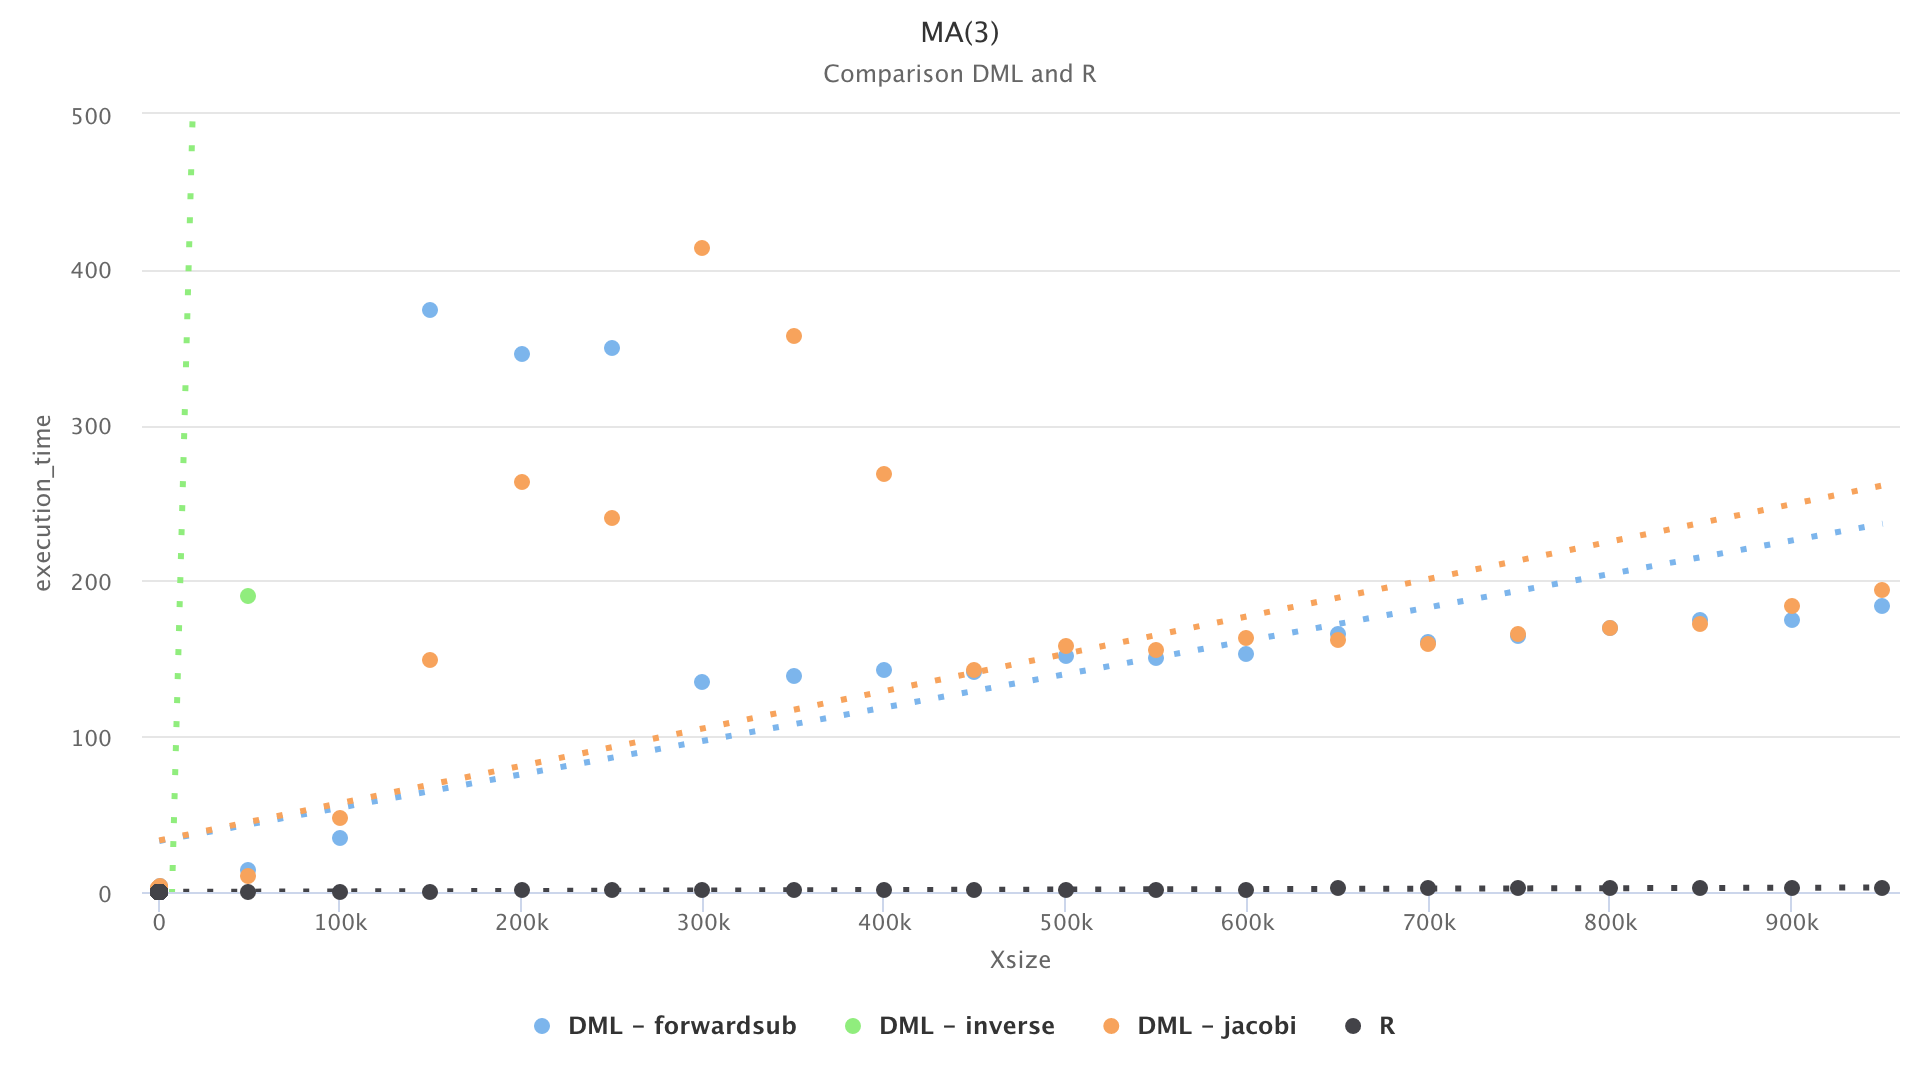
\includegraphics[width=\defaultsizeGraph]{images/ma3-exectime-scatter-all_reduced-regression.png}}
	\caption{\textbf{Execution time of MA(3) for DML and R for time series with sizes \textbf{up to $950,000$} }}
    \label{fig:ma3-exectime-scatter-all_reduced-regression}
\end{figure}

\begin{figure}[ht]
	\centering
	\scalebox{1}{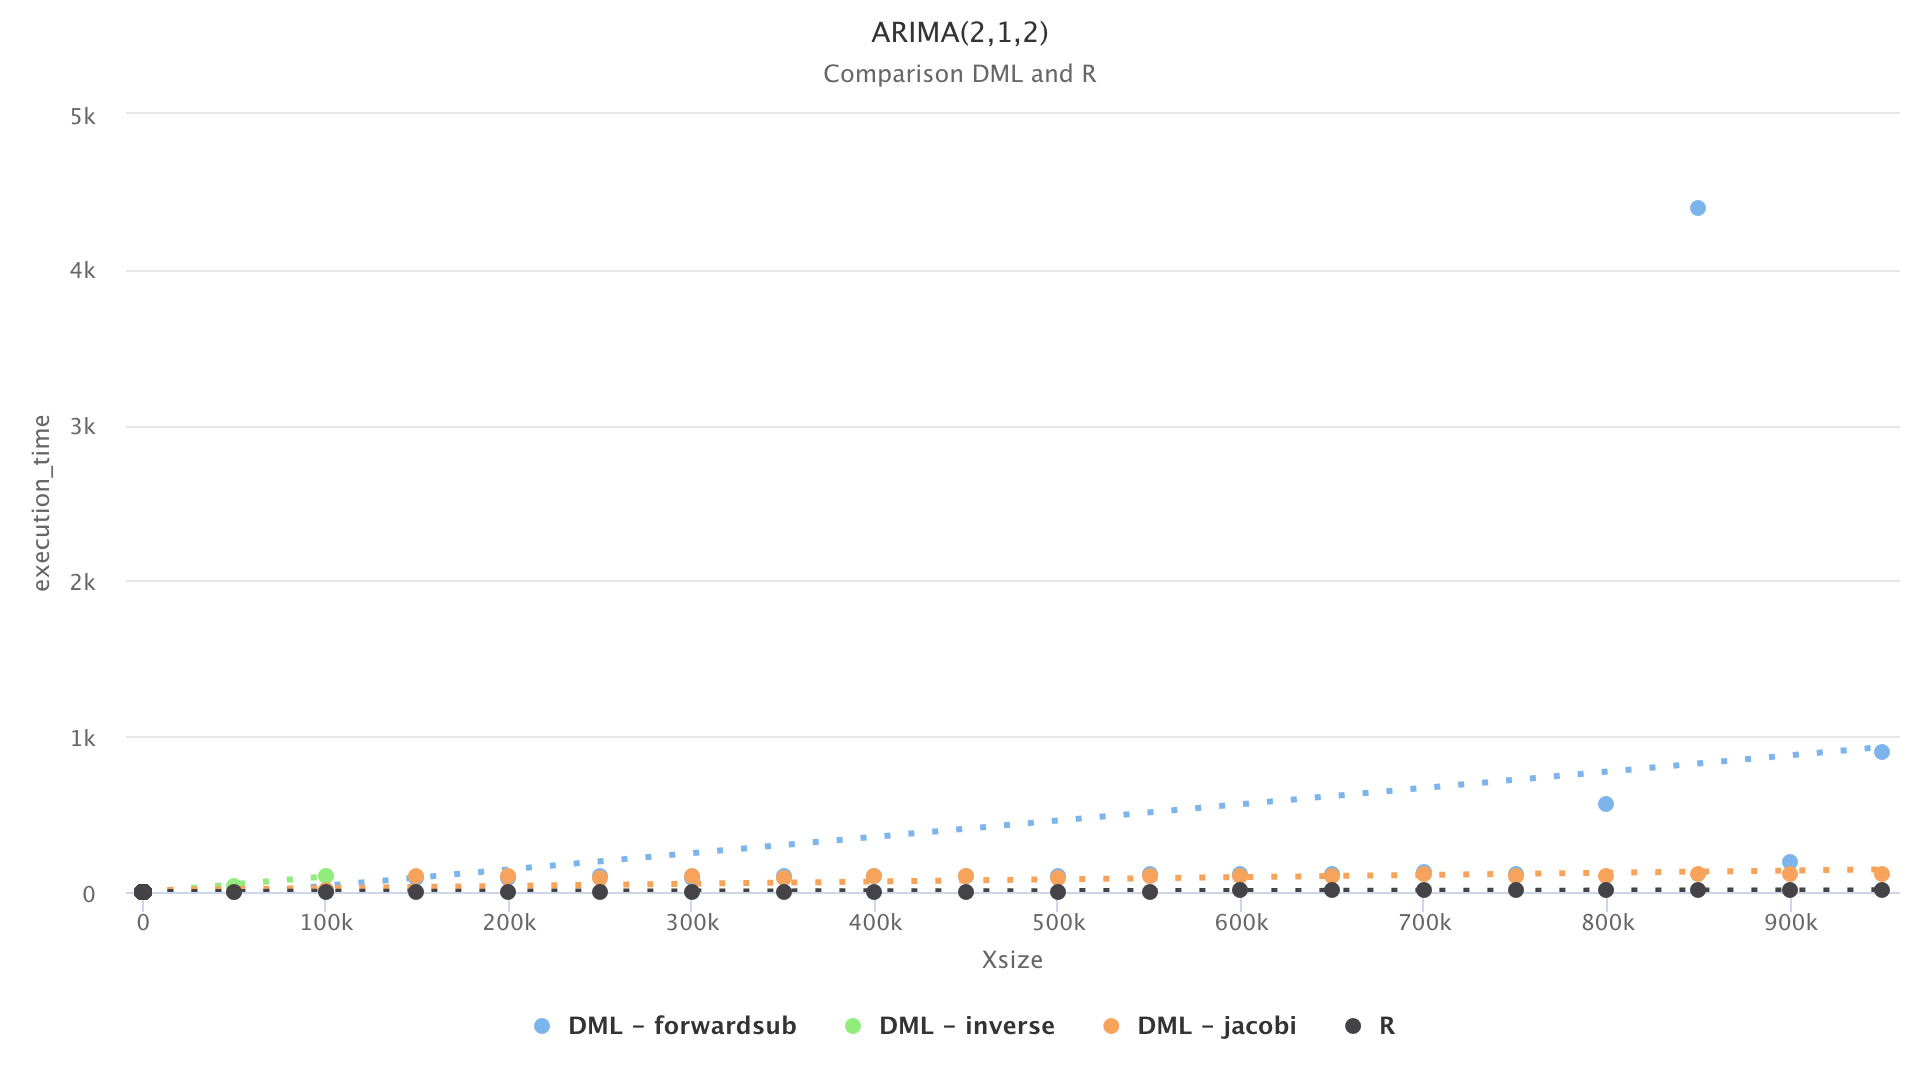
\includegraphics[width=\defaultsizeGraph]{images/arima212-exectime-scatter-all-regression.png}}
	\caption{\textbf{Execution time of ARIMA(2,1,2) for DML and R for time series with sizes \textbf{up to $950,000$} }}
    \label{fig:arima212-exectime-scatter-all-regression}
\end{figure}


\begin{figure}[ht]
	\centering
	\scalebox{1}{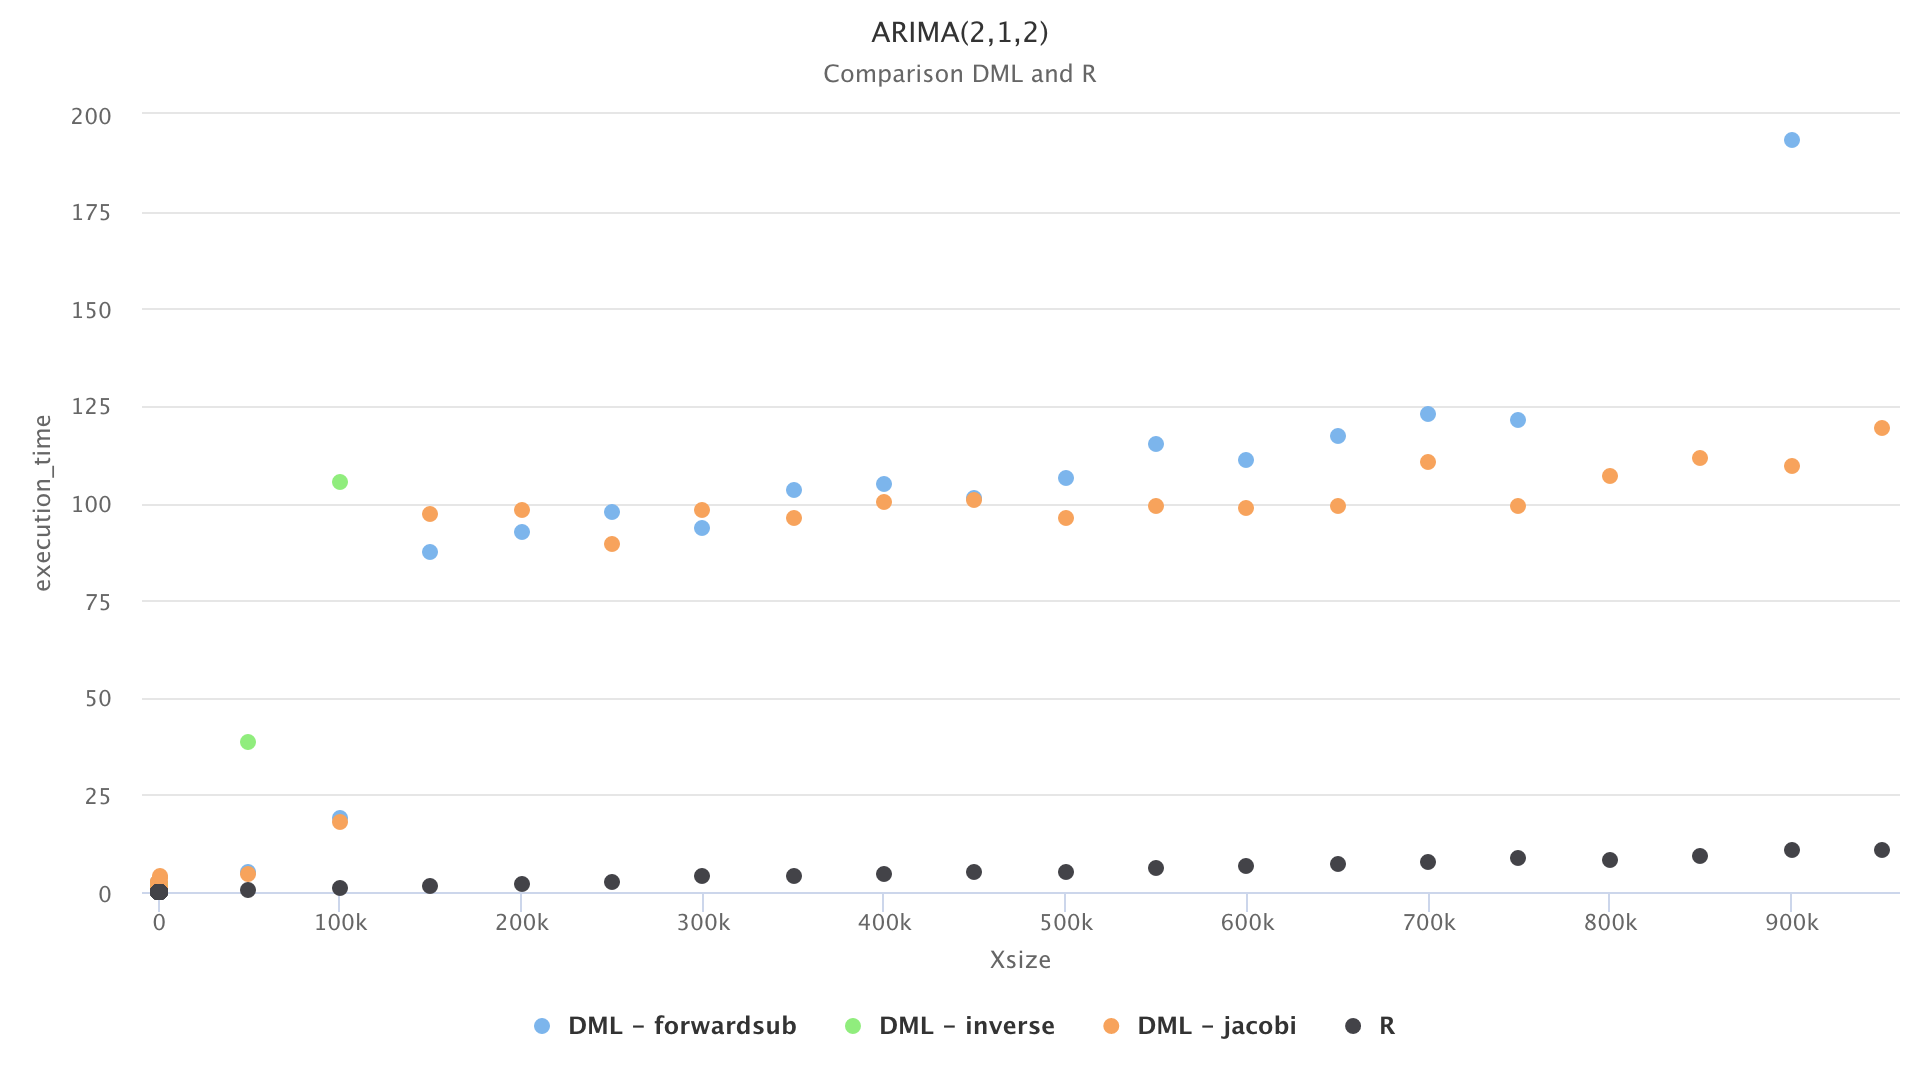
\includegraphics[width=\defaultsizeGraph]{images/arima212-exectime-scatter-all.png}}
	\caption{\textbf{Execution time} of ARIMA(2,1,2) for DML and R for time series with sizes \textbf{from $1,000$ to $950,000$} excluding outliers with an execution time greater than 200 seconds}
    \label{fig:arima212-exectime-scatter-all}
\end{figure}


\begin{figure}[ht]
	\centering
	\scalebox{1}{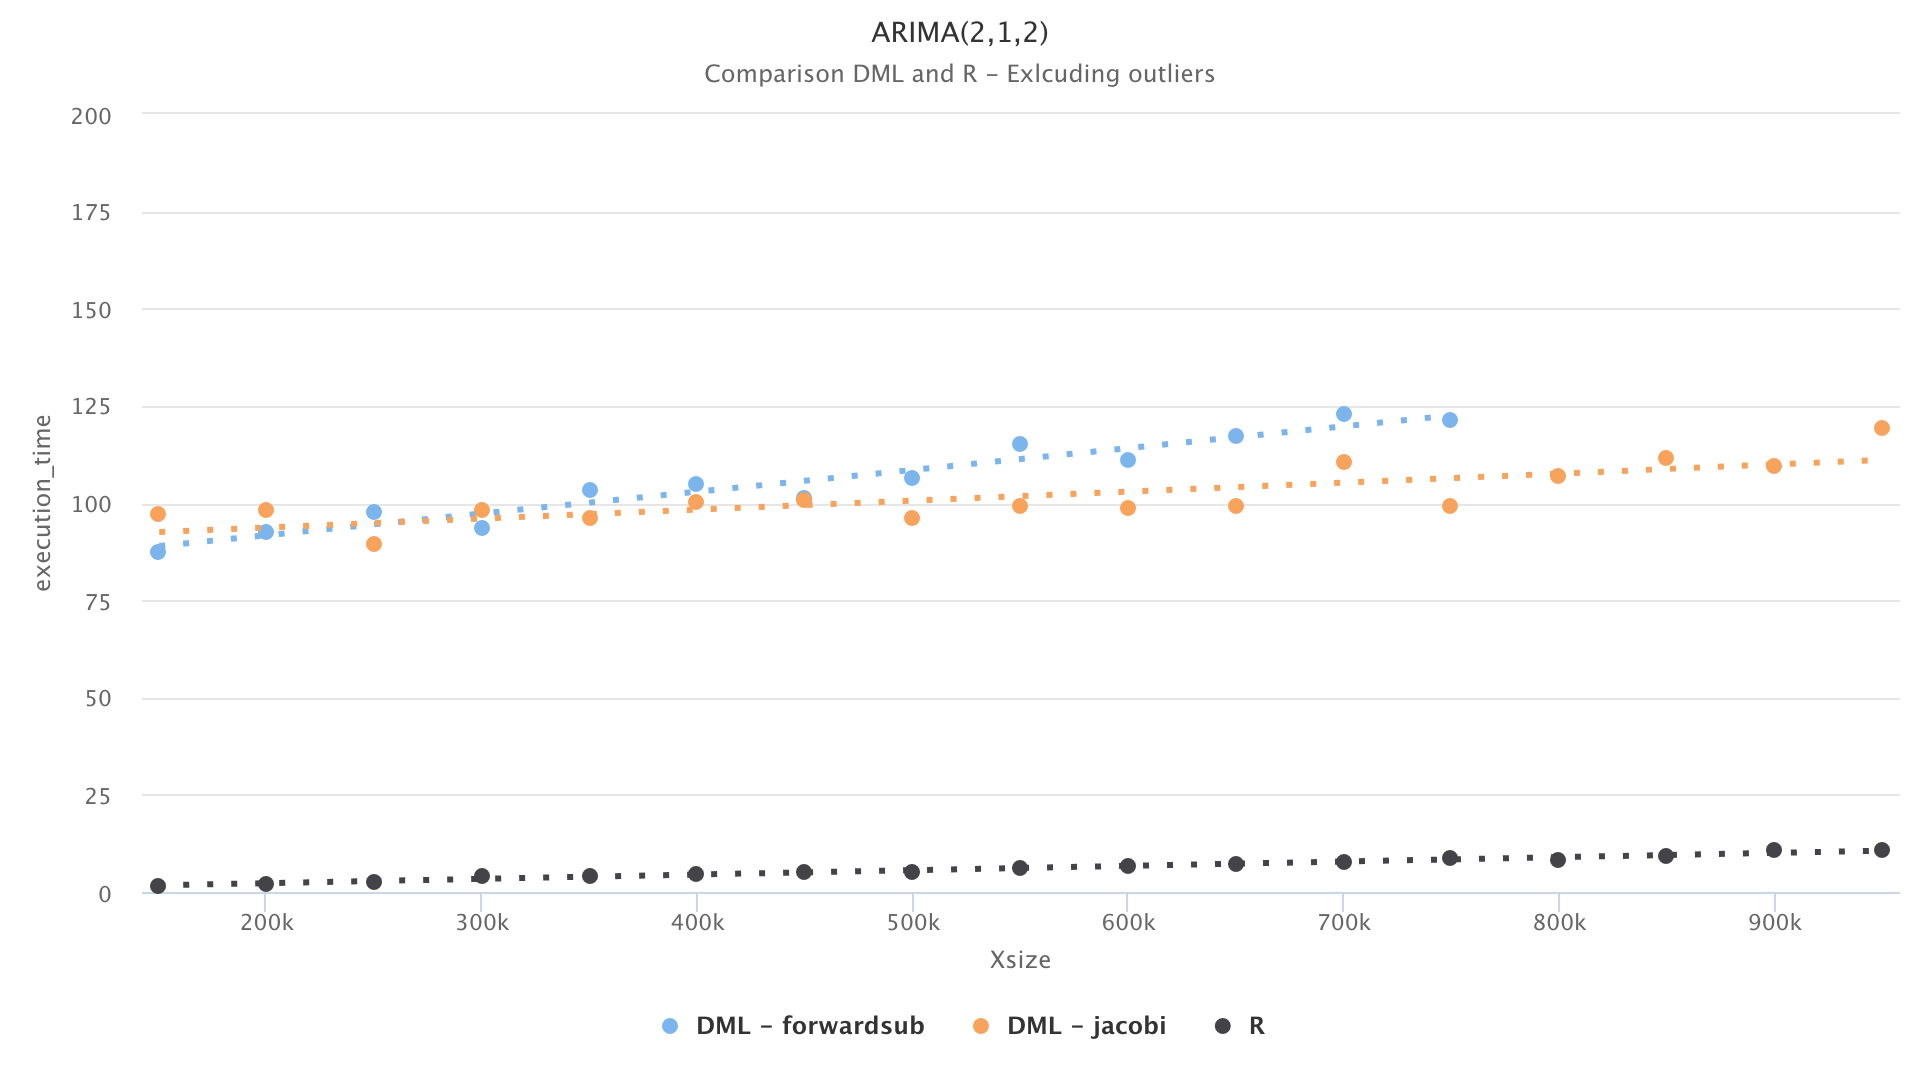
\includegraphics[width=\defaultsizeGraph]{images/arima212-exectime-scatter-all-excludeOutlier-regression.png}}
	\caption{\textbf{Execution time} of ARIMA(2,1,2) for DML and R for time series with sizes \textbf{from $100,000$ to $950,000$} excluding outliers with an execution time greater than 150 seconds}
    \label{fig:arima212-exectime-scatter-all-excludeOutlier-regression}
\end{figure}
